\chapter{\label{sec:filippov}Filippov-rendszerek}
A fejezet alapfogalmait di Bernardo és szerzőtársai \cite[2.2.3. szakasz]{dib} vezeti be; a relés szabályozás motivációját az 1.3.1. szakasz, a sliding bifurcations eseteit a 8. fejezet tárgyalja.


Tekintsük a
\begin{equation}
\dot{x}=\left\{
\begin{matrix}
F_1(x), \, \mathrm{ha} & H(x) > 0\\
F_2(x), \, \mathrm{ha} & H(x) < 0
\end{matrix}
\right.
\end{equation}
\noindent dinamikai rendszert. Feltesszük, hogy
$\left.F_1\right|_{H(x)=0} \neq \left.F_2\right|_{H(x)=0}$,
azaz a két vektormező határértéke eltér a felületen. Ez nem feltétlenül jelent különböző irányt. A
\begin{equation}
\Sigma=\{x:H(x)=0\}
\end{equation}
\noindent halmaz az úgynevezett \emph{kapcsolófelület}  (\textit{switching manifold}). Kapcsolófelületre mutat példát a \ref{fig:kapcsolofelulet}.~ábrán látható fekete szaggatott vonal.

A kör alakú határhoz most konkrét, dimenziótlan példát adunk. Legyen $x=(x_1,x_2)^\mathsf T$, és
\begin{equation}\label{eq:circle_switch_H}
H(x)=1-x_1^2-x_2^2.
\end{equation}
Így $\Sigma$ az egységkör, $H>0$ a kör belseje, $H<0$ a külseje. A két vektormező legyen
\begin{equation}\label{eq:circle_switch_fields}
F_1(x)=\begin{pmatrix}x_1\\-x_2\end{pmatrix}\quad(H>0),\qquad
F_2(x)=\begin{pmatrix}1\\-x_1\end{pmatrix}\quad(H<0).
\end{equation}
Belül tehát $\dot x_1=x_1$, $\dot x_2=-x_2$ nyeregtípusú mozgás, kívül $\dot x_1=1$, $\dot x_2=-x_1$ áramlás érvényes. A körön a két mező határértékei különböznek; az ottani folytatás szabályát a következőkben bevezetett Filippov-konstrukció adja meg. A \ref{fig:kapcsolofelulet}. ábrát közvetlenül ezekből a képletekből számítottuk újra.

\begin{figure}[htbp]
\centering
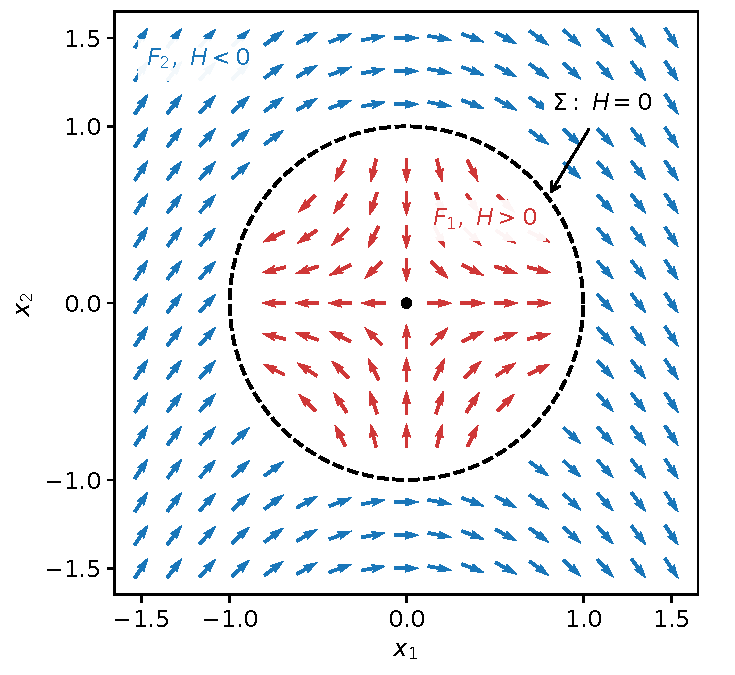
\includegraphics[width=.78\linewidth]{graphics_v3/circle_switch_fields.pdf}
\caption{Konkrét szakaszos vektormező a \eqref{eq:circle_switch_H}--\eqref{eq:circle_switch_fields} definíciókkal. Piros nyilak: $F_1$ a kör belsejében; kék nyilak: $F_2$ kívül. A fekete szaggatott kör $H=0$. A nyilak egységes hosszúságúak, csak az irányt jelölik; az origóban $F_1=0$.}
\label{fig:kapcsolofelulet}
\end{figure}

Továbbá bevezetjük
\begin{equation}
H_x=(\nabla H)^\mathsf{T}=\begin{pmatrix}
\frac{\partial H}{\partial x_1}&\frac{\partial H}{\partial x_2} &\dots
\end{pmatrix}
\end{equation}
\noindent deriváltat. A körpéldában $H_x=(-2x_1,-2x_2)$, amely az egységkörön sehol sem nulla, és befelé mutat, összhangban a belső tartományban pozitív $H$ választásával. A normális irányt $\nabla H$ adja, amely $H$ növekedése felé mutat. Feltesszük, hogy $H$ sima és $H_x\neq0$ a kapcsolófelületen; a jegyzetben $H_x$ sorvektor.

\emph{Attracting sliding region} néven jelöljük a $\Sigma$ kapcsolófelület azon részhalmazát, melyre $H_xF_1<0$ és $H_xF_2> 0$ skalárszorzat teljesül. Ezt a részhalmazt $\Sigma_s$-ként jelöljük, ahol $s$ index a $sliding$-ra utal. A sliding region területén a két dinamikai rendszerhez tartozó trajektóriák kapcsolófelületre merőleges komponensei egymás felé, azaz befelé mutatnak. Sliding region tartományra mutat példát a \ref{fig:csuszofelulet}.~ábra.

A \ref{fig:csuszofelulet}.~ábrán ugyanazokat a konkrét $H$, $F_1$ és $F_2$ függvényeket használjuk, mint a \ref{fig:kapcsolofelulet}.~ábrán. A normális komponensek:
\begin{equation}\label{eq:circle_normal_components}
\ell_1=H_xF_1=2(x_2^2-x_1^2),\qquad
\ell_2=H_xF_2=2x_1(x_2-1).
\end{equation}
Az egységkörön $\ell_1<0$ akkor teljesül, ha $|x_1|>|x_2|$, míg $\ell_2>0$ pontosan a bal félkörön. Ezért az attracting sliding region
\begin{equation}\label{eq:circle_sliding_arc}
\Sigma_s=\{(\cos\theta,\sin\theta):3\pi/4<\theta<5\pi/4\}.
\end{equation}
A két végpontban $\ell_1=0$, ezért ezek érintési pontok, és a szigorú egyenlőtlenségekkel definiált tartományhoz nem tartoznak hozzá. A zöld nyilak a lentebb levezetett $F_s$ sliding vektormező irányát mutatják. Például $x=(-1,0)$ esetén $\ell_1=-2$, $\ell_2=2$, így $\alpha=1/2$ és $F_s=(0,1/2)^{\mathsf T}$: a mozgás itt felfelé halad.

\begin{figure}[htbp]
\centering
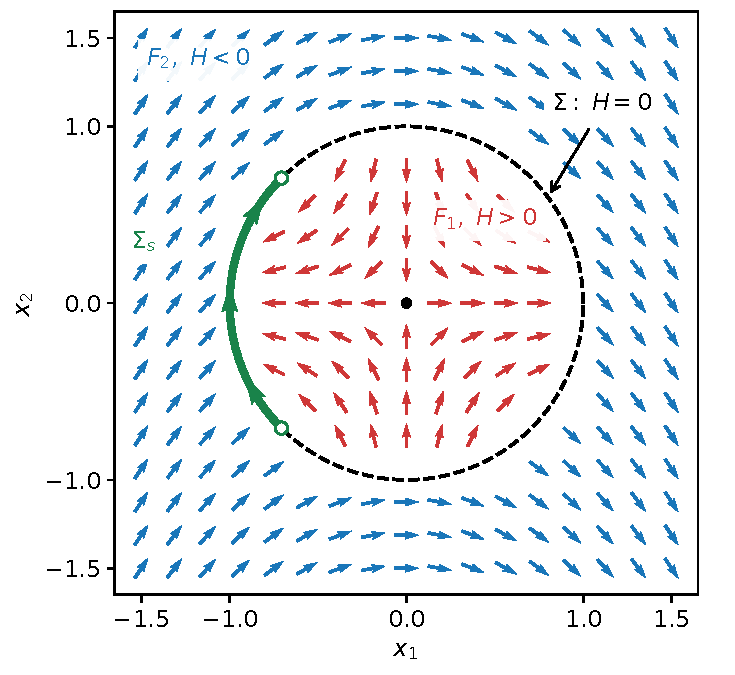
\includegraphics[width=.78\linewidth]{graphics_v3/circle_sliding_fields.pdf}
\caption{A \eqref{eq:circle_switch_H}--\eqref{eq:circle_switch_fields} mezőkhöz tartozó attracting sliding region (vastag zöld körív). A piros és kék nyilak $F_1$, illetve $F_2$, a zöld nyilak $F_s$ irányát mutatják; hosszuk nem sebességet jelöl. Az üres körök a tartomány végpontjai.}
\label{fig:csuszofelulet}
\end{figure}

A sliding region területén uralkodó dinamikát az
\begin{equation}
F_s=F_1(1-\alpha)+F_2\alpha
\end{equation}
\noindent egyenlet írja le. Vagyis lineárisan interpolálunk a két vektormező között oly módon, hogy $\alpha$-t úgy adjuk meg, hogy $H_xF_s=0$ teljesüljön. Ez akkor lesz igaz, ha $F_s$ és $H_x$ skaláris szorzata zérus:
\begin{equation}
H_xF_s =0 \,,
\end{equation}
\noindent tehát
\begin{equation}
H_xF_s = H_xF_1 (1-\alpha) + H_xF_2 \alpha = 0\,,
\end{equation}
\noindent melyből kifejezhető $\alpha$ értéke a következőképpen:
\begin{equation}
\alpha=\frac{H_xF_1}{H_x(F_1-F_2)}\,.
\end{equation}
A sliding dinamika a felület dimenziójára redukálódik, de általában nem szükségképpen egyszerű vagy stabil. Sliding mode control alkalmazásakor a kapcsolási törvényt és a felületet úgy tervezzük, hogy a felület elérhető legyen, és rajta a kívánt stabil dinamika alakuljon ki.

Jelölje $\ell_i=H_xF_i$ a normális komponenseket. Ha $\ell_1\ell_2>0$, transzverzális áthaladás történik. Az $\ell_1<0<\ell_2$ eset attracting sliding, míg $\ell_2<0<\ell_1$ repelling sliding: utóbbinál a felületre megszorított mező formálisan megadható, de az előrehaladó megoldás egyértelműsége külön vizsgálatot igényel. A $\ell_i=0$ határok érintési pontok. Attracting sliding esetén $0<\alpha<1$, így a kombináció konvex.

\section{Sliding mode control: munkahenger pozíciószabályozása}
\examplebody


Tekintsük a \ref{fig:munkahenger}.~ábrán látható elrendezést, mely munkahenger pozíciójának sliding mode control alapú szabályozására mutat példát. A hidraulikus tápegység (nyomásforrás) valamekkora $\Delta \tilde{p}>0$ konstans nyomást tud kiadni. A hengervezérlő szelep állásától függően a hidraulikus munkahengerbe $+\Delta \tilde{p}$ vagy $-\Delta \tilde{p}$ nyomás kerül. Ennek hatására a hengerfej jobbra vagy balra mozdul el. Célunk, hogy a munkahengert $x_{\rm k}$ kívánt pozícióba juttassuk a munkahenger sliding mode control alapú szabályozása által. Ehhez rendelkezésünkre áll egy PD szabályozó.

\begin{figure}[htbp]
\centering
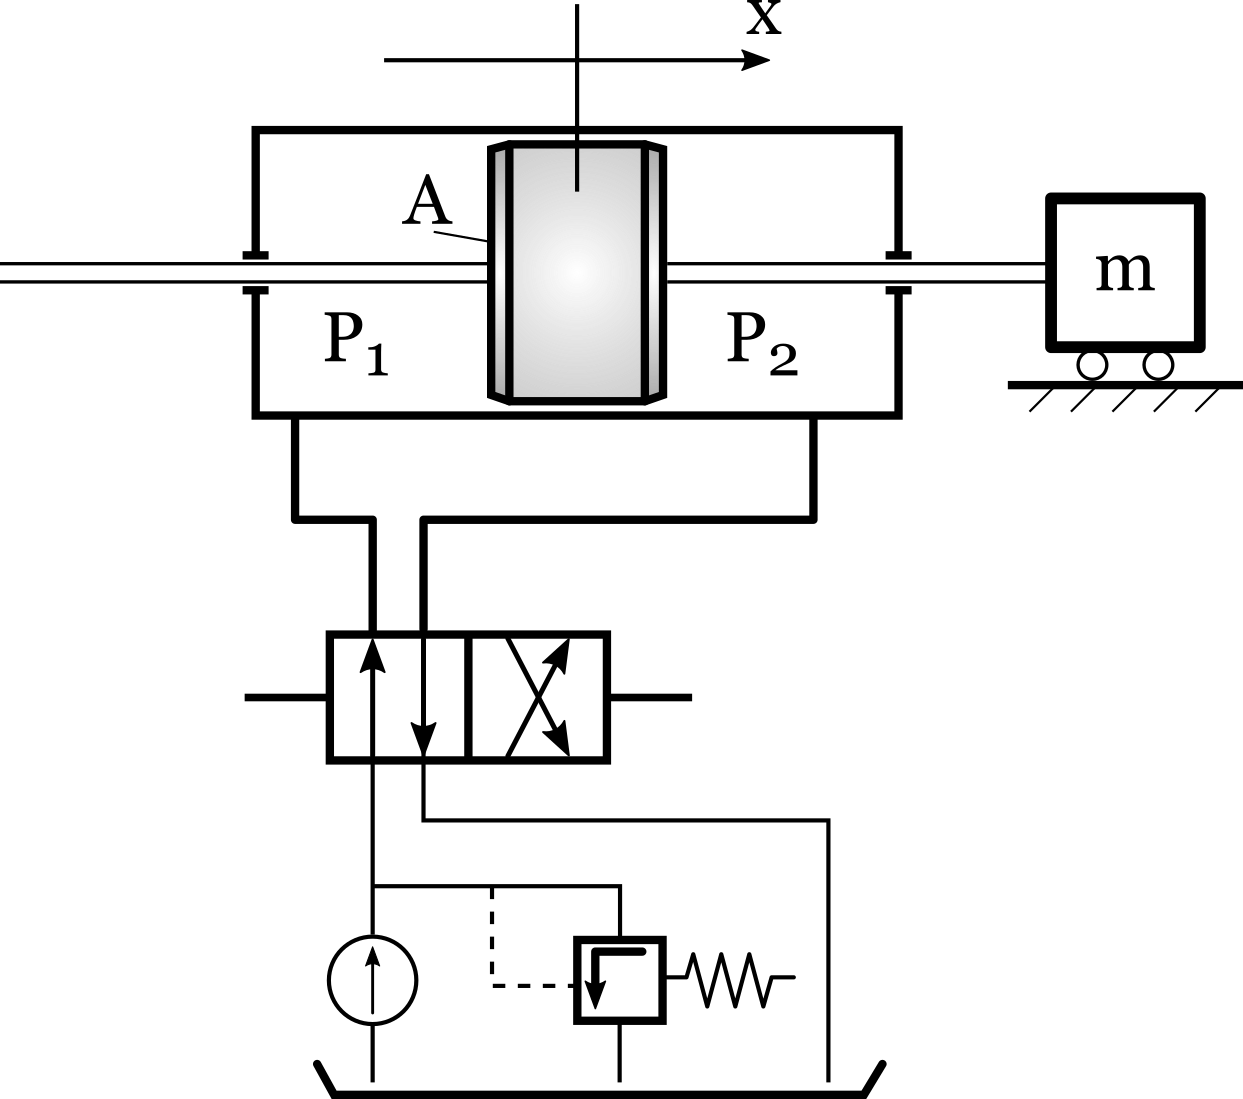
\includegraphics[width=0.5\textwidth]{graphics/munkahenger_fancy.png}
\caption{Munkahenger szabályozása.}
\label{fig:munkahenger}
\end{figure}

A dugattyú mozgását az alábbi másodrendű differenciálegyenlettel írhatjuk le:
\begin{equation}
m \ddot{x} + k \dot{x} = A \Delta p,
\end{equation}
\noindent ahol
\begin{equation}
	\Delta p = p_1- p_2 = \left\{
	\begin{matrix}
	+\Delta \tilde{p}, \mathrm{ha} & H(x) > 0\\
	-\Delta \tilde{p}, \mathrm{ha} & H(x) < 0
	\end{matrix}\,.
	\right.
\end{equation}
\indent A szabályozás során a munkahengert az $x_{\rm k} = 0$ pozícióba kívánjuk mozgatni. Ehhez a $H(x)$ függvényt egy PD szabályozási stratégia alapján írjuk elő:
\begin{equation} \label{eq:Hx}
H(x) = -P (x - x_{\rm k}) - D \dot{x} = -P x - D \dot{x},
\end{equation}
ahol az arányos és differenciáló tagok pozitívak: $P > 0$ és $D > 0$. A dinamikai rendszert az
\begin{equation}
x = (x_1 \; x_2)^{\rm T} = (x \; v)^{\rm T}
\end{equation}
\noindent változó bevezetésével elsőrendű alakra hozzuk. Ekkor a két vektormező a következő alakú:
\begin{equation}
F_1(x) = \left(
\begin{matrix}
x_2\\
\frac{A \Delta \tilde{p}}{m} - \frac{k}{m} x_2
\end{matrix}
\right), \quad
F_2(x) = \left(
\begin{matrix}
x_2\\
-\frac{A \Delta \tilde{p}}{m} - \frac{k}{m} x_2
\end{matrix}
\right).
\end{equation}
\noindent Mivel $\dot{x}=v=x_2$, a $H(x)$ által meghatározott kapcsolóvonal egyenlete a \eqref{eq:Hx}~egyenlet alapján
\begin{equation}
\Sigma = \left\{x: x_2 = -\frac{P}{D} x_1 \right\}\,,
\end{equation}
\noindent a kapcsolóvonalra merőleges irányt kijelölő $H_x$ gradiens pedig
\begin{equation}
H_x = \begin{pmatrix}-P&-D\end{pmatrix} \,.
\end{equation}

A kapcsolóvonal $\Sigma_{\rm s}$ sliding region része a
\begin{equation}
H_xF_1 = -P x_2 - \frac{D A \Delta \tilde{p}}{m} + \frac{D k}{m} x_2 < 0 \,,
\end{equation}
\noindent valamint az
\begin{equation}
H_xF_2 = -P x_2 + \frac{D A \Delta \tilde{p}}{m} + \frac{D k}{m} x_2 > 0
\end{equation}
\noindent egyenlőtlenségek által adott. Összevonva, még osztás nélkül:
\begin{equation}\label{eq:cylinder_sliding_condition}
-DA\Delta\tilde p<(Dk-Pm)x_2<DA\Delta\tilde p.
\end{equation}
Ha $Dk-Pm\neq0$, ebből a sliding region:
\begin{equation}
\Sigma_{\rm s} = \{x\in\Sigma: -x_2^* < x_2 < x_2^* \} \,,
\end{equation}
\noindent ahol
\begin{equation} \label{eq:x2csillag}
x_2^* = \frac{D A \Delta \tilde{p}}{|D k - P m|},\qquad Dk\neq Pm\,.
\end{equation}

A \eqref{eq:x2csillag} képlet ebben az esetben nem használható, mert nullával osztanánk. Ez azonban csak a tartomány végpontját megadó képlet korlátja: a vektormezők és a mozgásegyenletek továbbra is értelmesek. Visszatérve a \eqref{eq:cylinder_sliding_condition} osztás előtti feltételéhez, annak középső tagja minden véges $x_2$ esetén nulla. Mivel $D,A,\Delta\tilde p,m>0$, a két normális komponens
\begin{equation}\label{eq:cylinder_matched_normals}
H_xF_1=-\frac{DA\Delta\tilde p}{m}<0,\qquad
H_xF_2=+\frac{DA\Delta\tilde p}{m}>0.
\end{equation}
Tehát mindkét oldalról a kapcsolóvonal felé mutat a mező, annak minden pontjában:
\begin{equation}
\Sigma_s=\Sigma \qquad (Dk=Pm).
\end{equation}
Nincsenek véges végpontok. Az $x_2^*\to\infty$ határérték ezt a korlátlan kiterjedést fejezi ki, nem végtelen sebességet vagy szinguláris mozgást.

A kapcsolóvonal elérése is különösen egyszerűvé válik: a $\dot H=H_x\dot x$ azonosság és \eqref{eq:cylinder_matched_normals} alapján
\begin{equation}
\dot H=-\frac{DA\Delta\tilde p}{m}\operatorname{sgn}(H),\quad H\neq0,
\qquad
 t_{\rm el}=\frac{m|H(x(0))|}{DA\Delta\tilde p}.
\end{equation}
Az ideális modellben tehát minden véges kezdeti állapotból véges idő alatt elérjük a kapcsolóvonalat. Utána a Filippov-féle sliding megoldást kell használni, amely $H=0$-n tartja a pályát; itt nem a két klasszikus mező valamelyikét választjuk tartósan.

A két vektormezőt, a kapcsolófelületet és a sliding region tartományt szemlélteti a \ref{fig:csuszomod_szabalyozas}.~ábra.

\begin{figure}[ht]
\centering
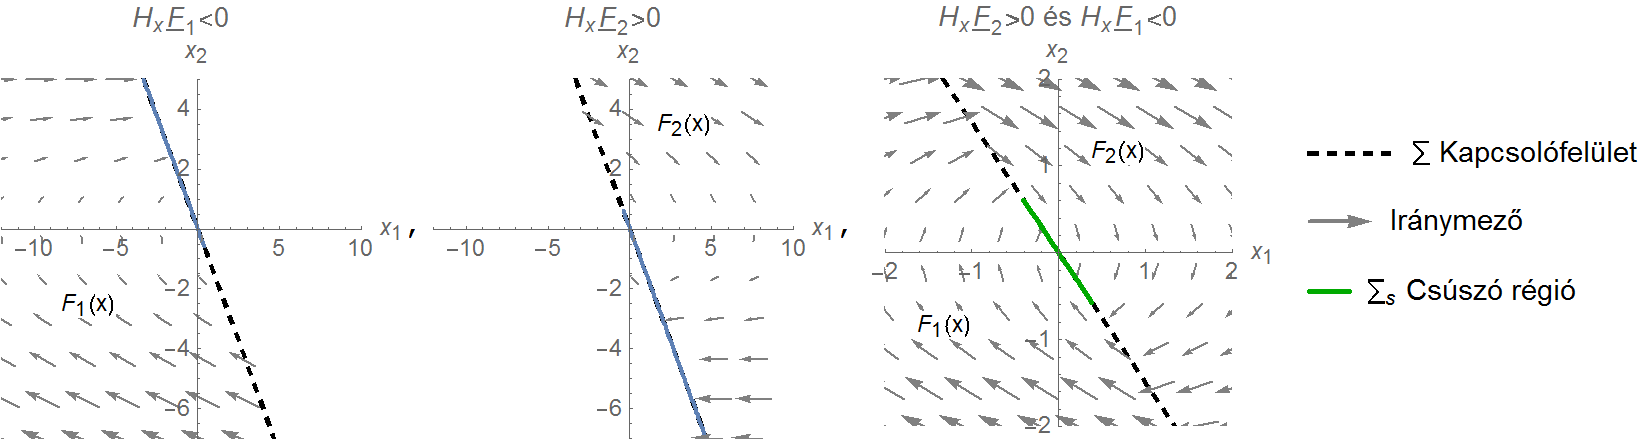
\includegraphics[width=\textwidth,trim={0.000bp 0.000bp 4.499bp 0.750bp},clip]{graphics/sliding_region_PELDA.png}
\caption{Munkahenger sliding mode control alapú szabályozása.}
\label{fig:csuszomod_szabalyozas}
\end{figure}

A $\Sigma_{\rm s}$-en érvényes dinamikát a korábban leírt
\begin{equation}
F_s = F_1 (1-\alpha) + F_2 \alpha
\end{equation}
\noindent vektormező határozza meg, ahol
\begin{equation}
\alpha = \frac{H_xF_1}{H_x(F_1-F_2)} = \frac{-P x_2 -D \left(\frac{A \Delta \tilde{p}}{m} - \frac{k}{m} x_2\right)}{-D \frac{2A \Delta \tilde{p}}{m}} \,.
\end{equation}
A nevező $H_x(F_1-F_2)=-2DA\Delta\tilde p/m$ nem nulla akkor sem, ha $Dk-Pm=0$: a Filippov-kombináció tehát ilyenkor is jól definiált. A keverési tényező egyszerűbb alakja
\begin{equation}
\alpha=\frac12-\frac{(Dk-Pm)x_2}{2DA\Delta\tilde p}.
\end{equation}
A különleges esetben $\alpha=1/2$ a teljes kapcsolóvonalon, vagyis $F_s=(F_1+F_2)/2$. A két ellentétes nyomáserő a konvex kombinációban kiegyenlíti egymást, és $\dot x_2=-(k/m)x_2$ marad. A $Dk=Pm$, azaz $P/D=k/m$ illesztés miatt éppen ez a csillapított mozgás tartja a pályát a kapcsolóvonalon.

Ezt $F_s$-be visszahelyettesítve, a kapcsolóvonalra megszorított dinamika
\begin{equation}
\begin{split}
F_s & = F_1 (1-\alpha) + F_2 \alpha = F_1 + \alpha (F_2-F_1) =  \\ & =
\begin{pmatrix}
x_2\\
\frac{A \Delta \tilde{p}}{m} - \frac{k}{m} x_2
\end{pmatrix} +
\alpha \begin{pmatrix}
0 \\
-\frac{2A \Delta \tilde{p}}{m}
\end{pmatrix} =
\begin{pmatrix}
x_2 \\
-\frac{P}{D}x_2
\end{pmatrix}
\end{split}
\end{equation}
\noindent vagyis
\begin{equation}
\left. \dot{x}_1 \right|_{\Sigma_s} = x_2, \qquad \left. \dot{x}_2 \right|_{\Sigma_s} = -\frac{P}{D} x_2.
\end{equation}

\underline{Megjegyzés:} $F_s$ második komponensét a $\Sigma$ kapcsolóvonal egyenletének idő szerinti deriválásával is meg lehet kapni.

A kapcsolóvonalon $x_2=-(P/D)x_1$, ezért a sliding megoldás exponenciálisan tart az origóhoz, $P/D$ lecsengési rátával. A sliding feltétele közvetlenül a két normális komponens előjeléből:
\[
|(Dk-Pm)x_2|<DA\Delta\tilde p.
\]
Pozitív fizikai paramétereknél és $Dk\neq Pm$ esetén tehát mindkét előjelű $Dk-Pm$ mellett létezik nemüres sliding region. A $Pm<Dk$ feltétel nem szükséges. Ha $Dk=Pm$, a teljes kapcsolóvonal attracting sliding region, de az origó elérése ettől nem válik pillanatszerűvé. A $t_{\rm el}$ elérési időtől kezdve
\begin{equation}
x_1(t)=x_1(t_{\rm el})e^{-(k/m)(t-t_{\rm el})},\qquad
x_2(t)=-\frac{k}{m}x_1(t).
\end{equation}
A kapcsolóvonalat tehát véges idő alatt érjük el, az origóhoz pedig általában csak aszimptotikusan tartunk; a lecsengés időállandója $m/k=D/P$.

A $P/D$ arány növelése gyorsítja a sliding dinamika lecsengését, de a tartomány mérete $1/|k-mP/D|$ szerint változik: először növekedhet, majd a $P/D=k/m$ érték fölött csökken. Véges pozitív paramétereknél nem tűnik el. A \ref{table:parameter}. táblázat értékeivel $Pm=0{,}21$, $Dk=0{,}02$, és $x_2^*\approx0{,}5263\,\mathrm{m/s}$, ami összhangban van a sliding lehetőségével.

Szimulációs példát mutat a \ref{fig:sliding_mode_control}.~ábra. A szimuláció során felhasznált paraméterértékeket a \ref{table:parameter}.~táblázat tartalmazza. $x_1(0) = -12$~m és $x_2(0) = 0.2$~m/s kezdeti feltételekkel indítva a szimulációt, a kapcsolófelületen áthaladva, a sliding region tartományba kerül a megoldás, majd a rendszer a kapcsolóvonalon tart a $(0 \; 0)^{\rm T}$ egyensúlyi helyzethez.
\begin{table}[htbp]
	\caption{Paraméterértékek}
	\vspace{0.1 cm}
	\centering
	\begin{tabular}{|c|c|c|c|c|c|} \hline
	$P$ [1/s] & $D$ [1] & $m$ [kg] & $A$ $[{\rm m}^2]$ & $\Delta \tilde{p}$ [Pa] & $k$ [Ns/m] \\ 	\hline
	$0.3$ & $0.2$ & $0.7$ & $0.5$ & $1$ & $0.1$ \\ \hline
	\end{tabular}
	\label{table:parameter}
\end{table}
\begin{figure}[ht]
\centering
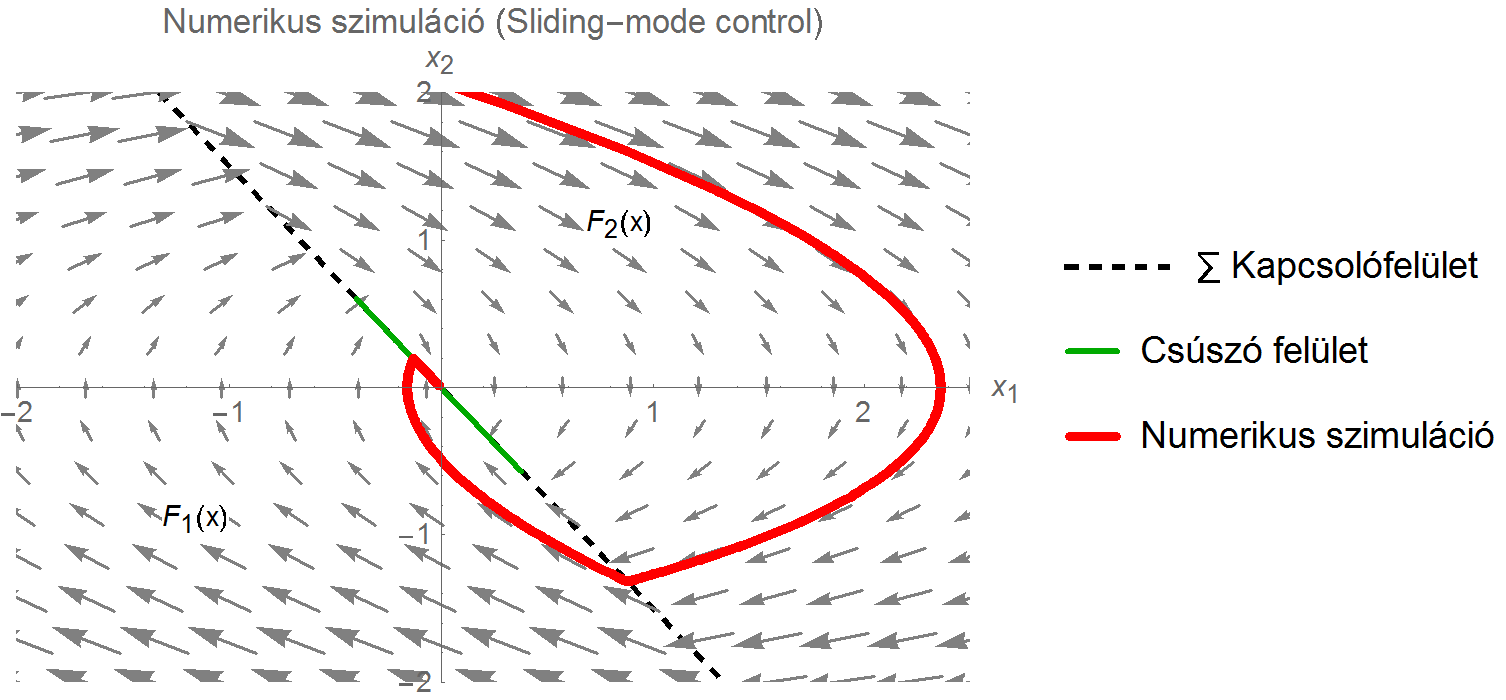
\includegraphics[width=\textwidth,trim={0.000bp 2.250bp 5.249bp 2.250bp},clip]{graphics/sliding_mode_control.png}
\caption{A sliding mode control által eredményezett trajektória. Kezdeti feltételek: $x_1(0) = -12$~m, $x_2(0) = 0.2$~m/s.}
\label{fig:sliding_mode_control}
\end{figure}
\exampleend

